\section{Dual Phase Considerations for Calibration}
\label{sec:DP}

%The DUNE \dword{dpmod} design has some unique features that require special considerations for calibration. 
Some unique features of the DUNE \dword{dpmod} design require special considerations regarding calibration. These features include the single vertical \SI{12}{\m} long drift, gain of the \dwords{lem}, ion accumulation at the liquid-gas interface, and the \lar flow pattern. All of these can amplify the nominal space-charge effect expected in the \detmodule. 

While space charge from cosmic rays is expected to be negligible in both %single and dual phase detectors
\spmod and \dpmod, other ionization sources such as ${^{39}}$Ar can result in non-negligible E field and spatial distortions. Simulation studies have shown that the space charge from ${^{39}}$Ar is more pronounced for \dword{dp} especially for spatial distortions (at the \SI{5}{\cm} level with a \num{2} to \num{3}\% impact on %dQ\/dx 
$dQ/dx$ via recombination) as shown in Figure~\ref{fig:scedp}. The
%argon 
\lar flow pattern can amplify space-charge effects as well, which may be significant for \dual (as well as \single).

\begin{dunefigure}[Simulated effects of space charge on distortions in reconstructed ionization electron cluster positions in a \dpmod{} ]
{fig:scedp}
{Illustration of the simulated effects of space charge on distortions in reconstructed ionization electron cluster positions in the %DUNE dual phase FD. 
\dpmod. Results are shown for the effect in $x$ (left) and $y$ (right). The distortions in reconstructed ionization-electron cluster position are shown in units of \si{\centi\m} and are plotted as a function of the true position in the TPC. Simulation results are shown for a central slice in $z$. APA corresponds to $x=0$ and CPA corresponds to $x=12$\si{\m}.}
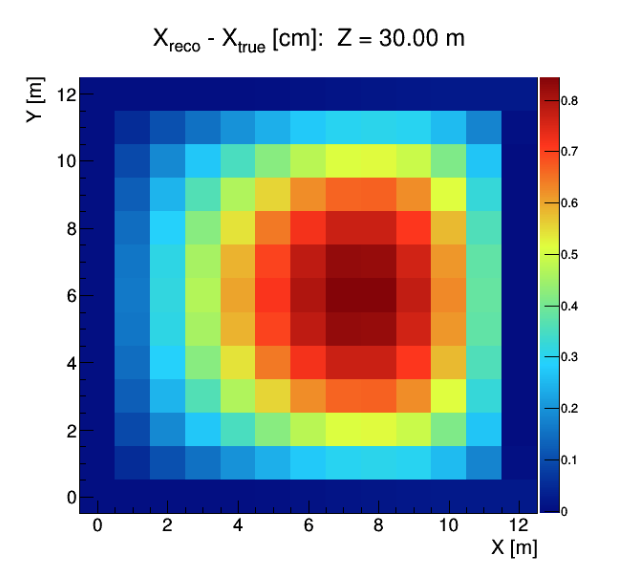
\includegraphics[width=.49\textwidth]{sce_x.png}
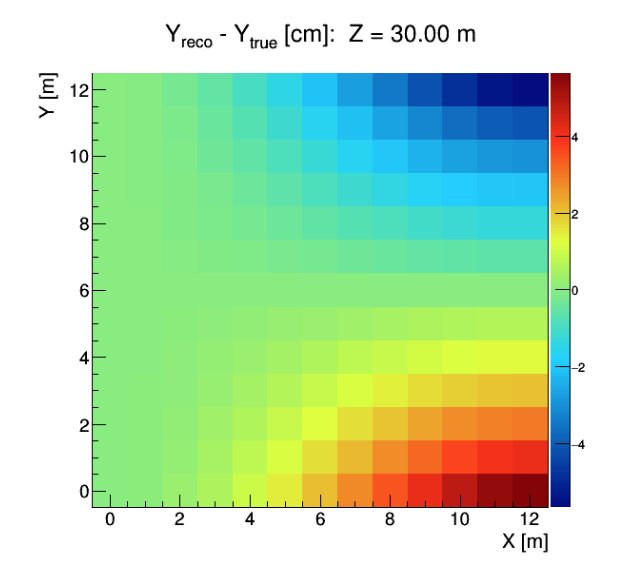
\includegraphics[width=.49\textwidth]{sce_y.png}
\end{dunefigure}

The gain of the \dwords{lem} will also need to be calibrated in the \dpmod. Any error in the charge gain in the LEM will directly impact the energy uncertainty for electromagnetic showers. The LEM gain is sensitive to many factors such as the hole size, copper rim offset, board thickness, hole inner surface conductivity, charging effects, and extraction and collection field (gap between electrodes). 
A gain map of the entire LEM surface will be needed, and if the gain drifts with time, periodic re-mapping of the gain may be needed. Furthermore, it is unclear how the charge and discharge cycles (e.g., due to a \SI{12}{\m} vertical cosmic track) impact the stability of gain. Additionally, a reduced gain can result in much stricter requirements on the electron lifetime. 

An additional complication for \dual involves positive ions collecting above the liquid-gas interface and creating surface interface issues which can lead to significant spatial distortions. If the electron lifetime is poor, it can result in electrons being captured by impurities, forming negative ions that can drift up toward the LEM. If these negative ions (or the electrons stripped off these ions) cannot be extracted into the gas phase by the extraction field, the  
negative ions will build up at the liquid surface forming non-uniform negative surface charge. This non-uniform negative surface charge will distort the electron drift path; %can 
it may also change the extraction field and alter the gain of LEMs in gaseous argon.% \fixme{gas gain?} resolved

The size of this effect needs to be understood and possibly calibrated. The \dword{pddp}, given its size, would %\fixme{will be an excellent test bench?}
be an excellent test bench to observe all the effects mentioned in this section. More dedicated studies will be planned in this direction with the \dword{pddp} group.